\documentclass[]{article}
\usepackage[spanish.mexico]{babel}
\usepackage[T1]{fontenc}
\usepackage[utf8]{inputenc}
%\usepackage{lmodern}
\usepackage[a4paper]{geometry}

%Plotting

\usepackage{pgfplots}
\pgfplotsset{width=10cm,compat=1.9} 
%\usepgfplotslibrary{external}
%\tikzexternalize 

%Graficos e imagenes
\usepackage{graphicx}
%\graphicspath{ Imagenes/ }

\usepackage{natbib}
%\usepackage{cite}

\usepackage{subcaption}

%Grafico de barras
%\usepackage{pgfplots}


\usepackage{tikz}
\usepackage[american voltages, american currents,siunitx]{circuitikz}

\title{Máquina de propósito general Luken}
\author{Pablo Vivar Colina}
%\date{Mayo 2018}


\begin{document}
	
%%\usepackage[top=2cm,bottom=2cm,left=1cm,right=1cm]{geometry}


\begin{titlepage}
     \begin{center}
	
\includegraphics[width=0.09\textwidth]{UNAM}\Large Universidad Nacional Autónoma de México
        	
\includegraphics[width=0.09\textwidth]{FI}\\[2cm]
        \Large Facultad de Ingeniería\\[2cm]
       % \Large División de Ciencias Básicas\\[1cm]
         \Large Laboratorio de Diseño Digital (6748)\\[2cm]
         %la clave antes era:4314
         \footnotesize Profesor: Ing. Armando Rojas Ascencio\\[2cm]
        \footnotesize Semestre 2020-1\\[2cm]
        
       

        \Large Práctica No. 7\\[2cm]
        
           

\Large Aplicaciones con circuitos combinacionales
        
         %Texto a la derecha
          \begin{flushright}
\footnotesize  Grupo 1\\[0.5cm]
\footnotesize Brigada: 1\\[0.5cm]
\footnotesize Gómez Álvarez Gustavo Alejandro\\[0.5cm]
\footnotesize Vivar Colina Pablo\\[0.5cm]
 \end{flushright}
    %Texto a la izquierda
          \begin{flushleft}
        \footnotesize Ciudad Universitaria Septiembre de 2019.\\
          \end{flushleft}
         
          
        %\vfill
        %\today
   \end{center}
\end{titlepage}
 %agregar portada

\maketitle

%\tableofcontents  % Write out the Table of Contents

%\listoffigures  % Write out the List of Figures

\section{Seguridad en la ejecución}

\begin{table}[h!]
	\begin{tabular}{|c|c|c|}
		\hline
		\textbf{Peligro o Fuente de energía} & \textbf{Riesgo asociado}     & \textbf{}      \\ \hline
		1                                    & Manejo de Corriente Alterna  & Electrochoque  \\ \hline
		2                                    & Manejo de Corriente Continua & Daño al Equipo \\ \hline
	\end{tabular}
\end{table}

\section{Objetivos de aprendizaje}

Aprender el manejo del equipo de laboratorio, código de resistores, tableta de prototipos y cables adecuados para cada equipo.\\
Comprobar la ley de ohm y las leyes de Kirchhoff.\\
Medición de diferentes parámetros, mediante circuitos resistivos: Voltaje, corriente, impedancia, frecuencia, periodo, fase y magnitud.\\

\section{Material y Equipo}

\begin{itemize}
	 
	 \item Osciloscopio, generador de funciones, fuente de poder y multímetro.
	 \item Cables, tableta de prototipos (Breadboard), diodos LED.
	 \item Compuertas AND, OR, NAND, NOR.
	 
\end{itemize}

\section{Actividad de investigación previa}


\section{Orden de Drivers}


\begin{figure}
	\centering
	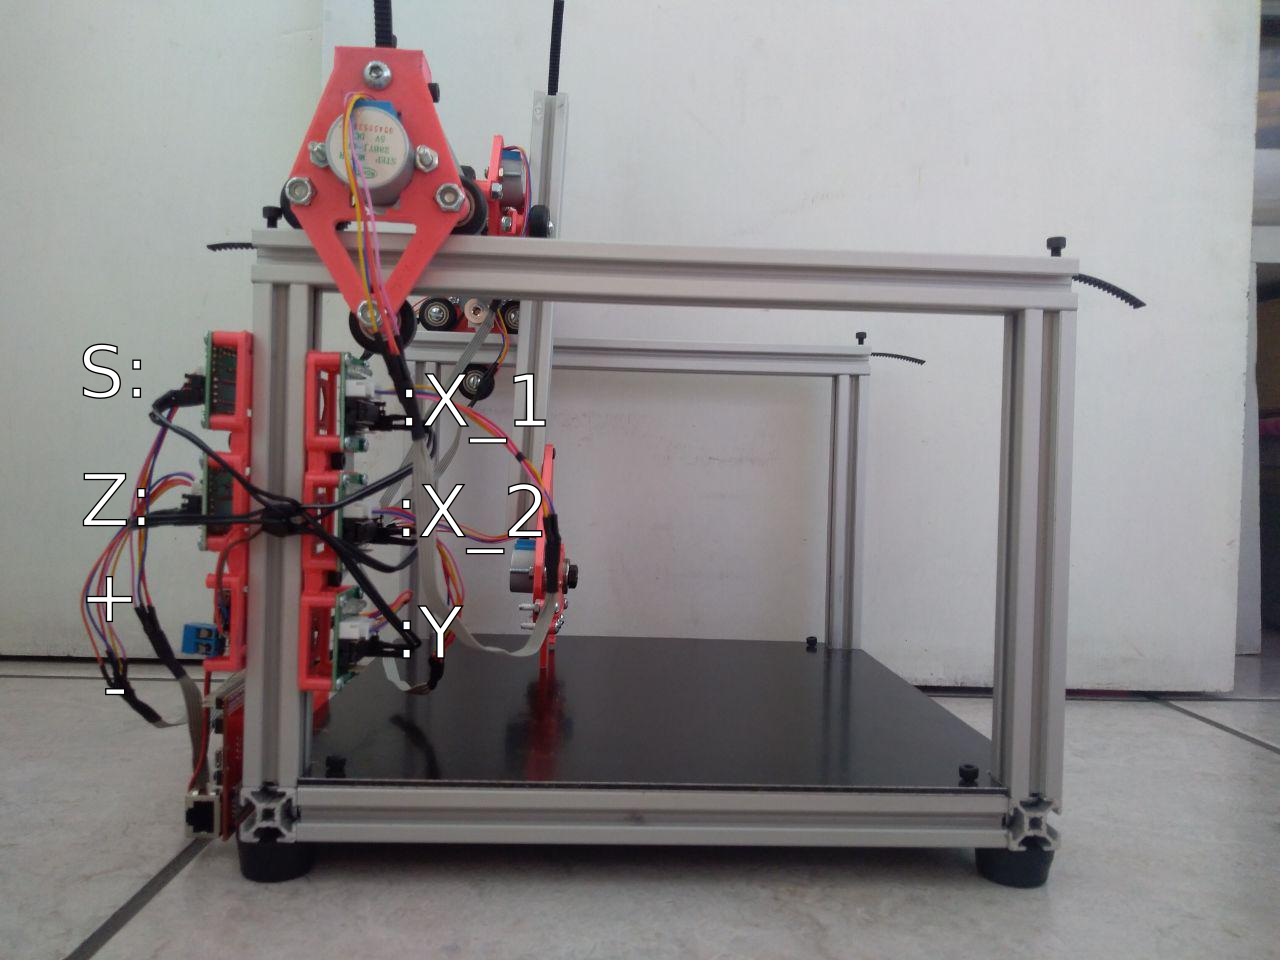
\includegraphics[width=0.8\textwidth]{DriversLabel}
	\caption{Disposición de módulos drivers}
	\label{fig:circuitoFisico}
\end{figure}


%\section{Referencias}

\bibliographystyle{plain}
\bibliography{Referencias.bib}



\end{document}
